\chapter{Projeto proposto: Enriquecimento de contexto de entidades no tempo}

Tendo agora explorado de maneira relativamente detalhada as diferentes etapas do sistema completo proposto por este trabalho, podemos isolar algumas partes e focar em alguns detalhes de implementação da etapa de enriquecimento de contexto que imaginamos ser cruciais para o alcance de resultados excelentes na modelagem de contexto semântico propriamente dita.

\section{Metodologia}

Serão descritas duas abordagens, ambas sujeitas a todas as etapas do sistema completo exceto a de enriquecimento de contexto: \textbf{coleta} de múltiplas fontes de dados; \textbf{processamento} de múltiplas camadas de dados; e \textbf{aplicação} do conhecimento extraído em recomendação de conteúdo e agentes virtuais. 

\begin{itemize}
    \item Consideraremos como \textbf{abordagem clássica}, aquela que faz uso de apenas um tipo de canal de dados por vez durante a aplicação, pois não contempla uma camada de enriquecimento multidimensional de contexto.
    \item  Por outro lado, descrevemos como \textbf{abordagem multidimensional} aquela que faz uso de todas as técnicas descritas no capítulo \ref{c:enriquecimento_de_contexto} para fornecer uma definição de contexto rica à camada de aplicação.
\end{itemize}

Espera-se ser possível identificar com facilidade a fragilidade da \textbf{abordagem clássica} e os benefícios da \textbf{abordagem multidimensional} a partir dos modelos expostos neste capítulo.

\newpage

\section{Fluxo de processamento}

O fluxo de processamento, em cada um dos cenários, é representado a seguir:

\begin{figure}[h]
\caption{abordagem clássica}
\centering
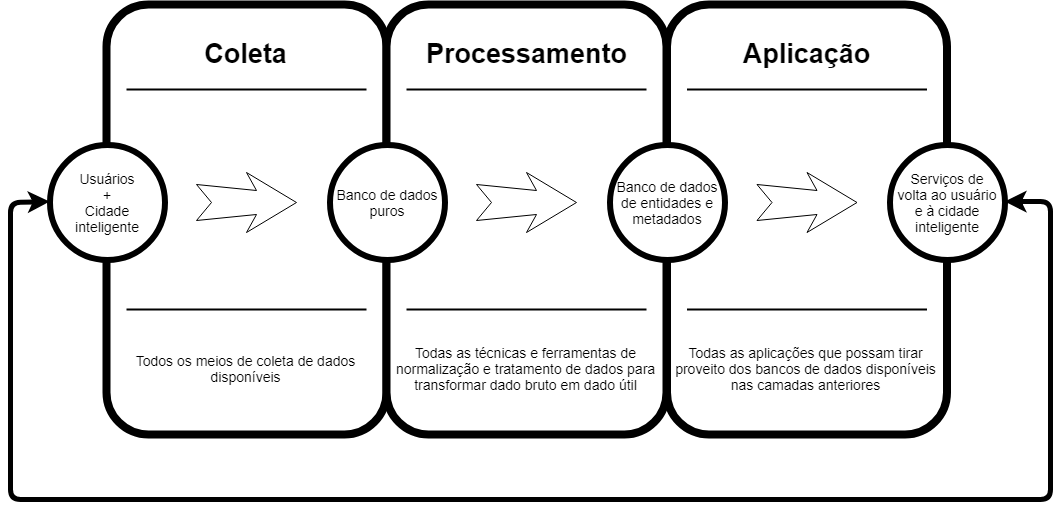
\includegraphics[width=0.8\textwidth]{images/PoorFlow.png}
\end{figure}

\begin{figure}[h]
\caption{abordagem multidimensional}
\centering
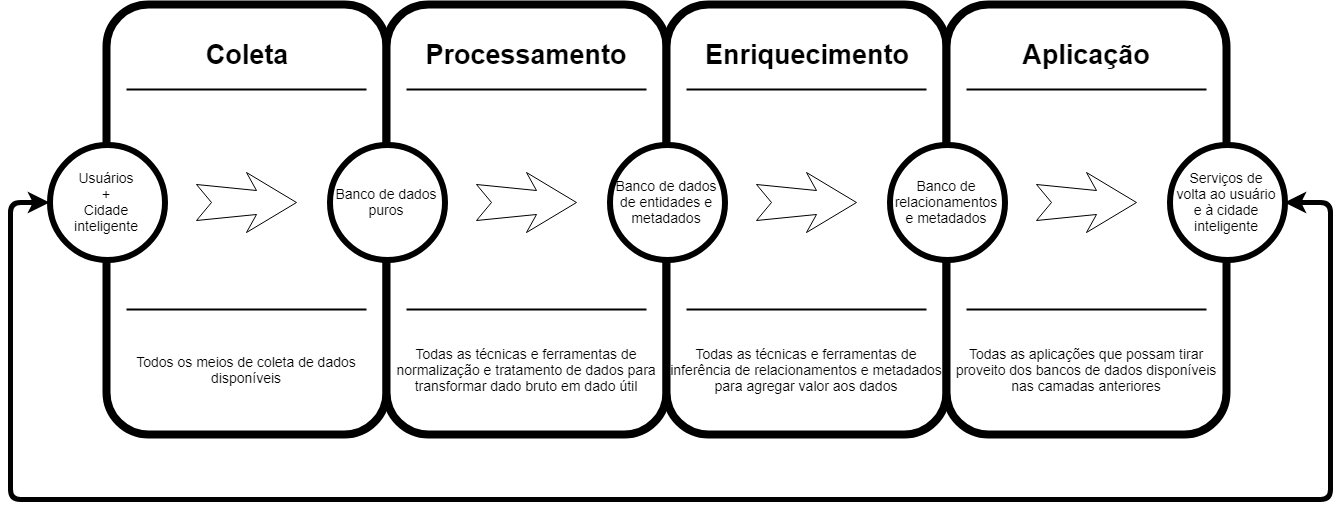
\includegraphics[width=0.8\textwidth]{images/FullFlow.png}
\end{figure}

\section{Estrutura das representações de contexto}

Apesar dos detalhes das etapas do fluxo terem sido descritas anteriormente, a camada de aplicação pode ser considerada agnóstica quanto à implementação dos bancos de dados de entidades, metadados e relacionamentos. Com isso, podemos considerar que a estrutura da representação de contexto de cada um dos cenários confia nas camadas anteriores de maneira transparente.

